\chapter{Results}
\label{results}

\minitoc

In this chapter relevant articles gathered on ...

\newpage

\section{Introduction and Clarification}

\begin{table}[H]
\begin{center}
    \begin{tabular}{| p{5cm} | p{3.7cm} | p{1cm} | p{4cm} |}
    \hline
    \textbf{Article Name} & \textbf{Author(s)} & \textbf{Year} & \textbf{Keywords} \\ \hline
    Inter-team Coordination in Large-scale Globally Distributed Scrum: Do Scrum-of-Scrums Really Work? & Maria Paasivaara, Casper Lassenius, Ville T. Heikkilä & 2012 & Agile Software Development; Distributed Scrum; Global Software Engineering; Inter-team Coordination \\ \hline
    Communities of Practice in a Large Distributed Agile Software Development Organization – Case Ericsson & Maria Paasivaara, Casper Lassenius & 2014 & Communities of Practice; Large-scale Agile Software Development; Scaling Agile \\ \hline
    Operational Release Planning in Large-scale Scrum with Multiple Stakeholders – A Longitudinal Case Study at F-Secure Corporation & Ville T. Heikkilä, Maria Paasivaara, Kristian Rautiainen, Casper Lassenius, Towo Toivola, Janne Järvinen & 2015 & Agile Software Development; Scrum; Large Projects; Release Planning; Software Project Management \\ \hline
Towards a Governance Framework for Chains of Scrum Teams & Jan Vlietland, Hans van Vliet & 2015 & Agile; Chain of Scrum Teams; Coordination; Priority; Alignment; Predictability \\ \hline
    \end{tabular}
    \caption{Summary of articles used in this chapter.}
    \label{soauitc}
\end{center}
\end{table}

\begin{table}[H]
\begin{center}
    \begin{tabular}{| p{4cm} | p{8cm} |}
    \hline
    \textbf{Role} & \textbf{Description of role} \\ \hline
    Scrum master & \\ \hline
    Functional architect & \\ \hline
    Technical architect & \\ \hline
    Tester & \\ \hline
    Developer & \\ \hline
    \end{tabular}
    \caption{Team roles present in Scrum teams.}
    \label{trpist}
\end{center}
\end{table}

\begin{figure}[H]
\centering
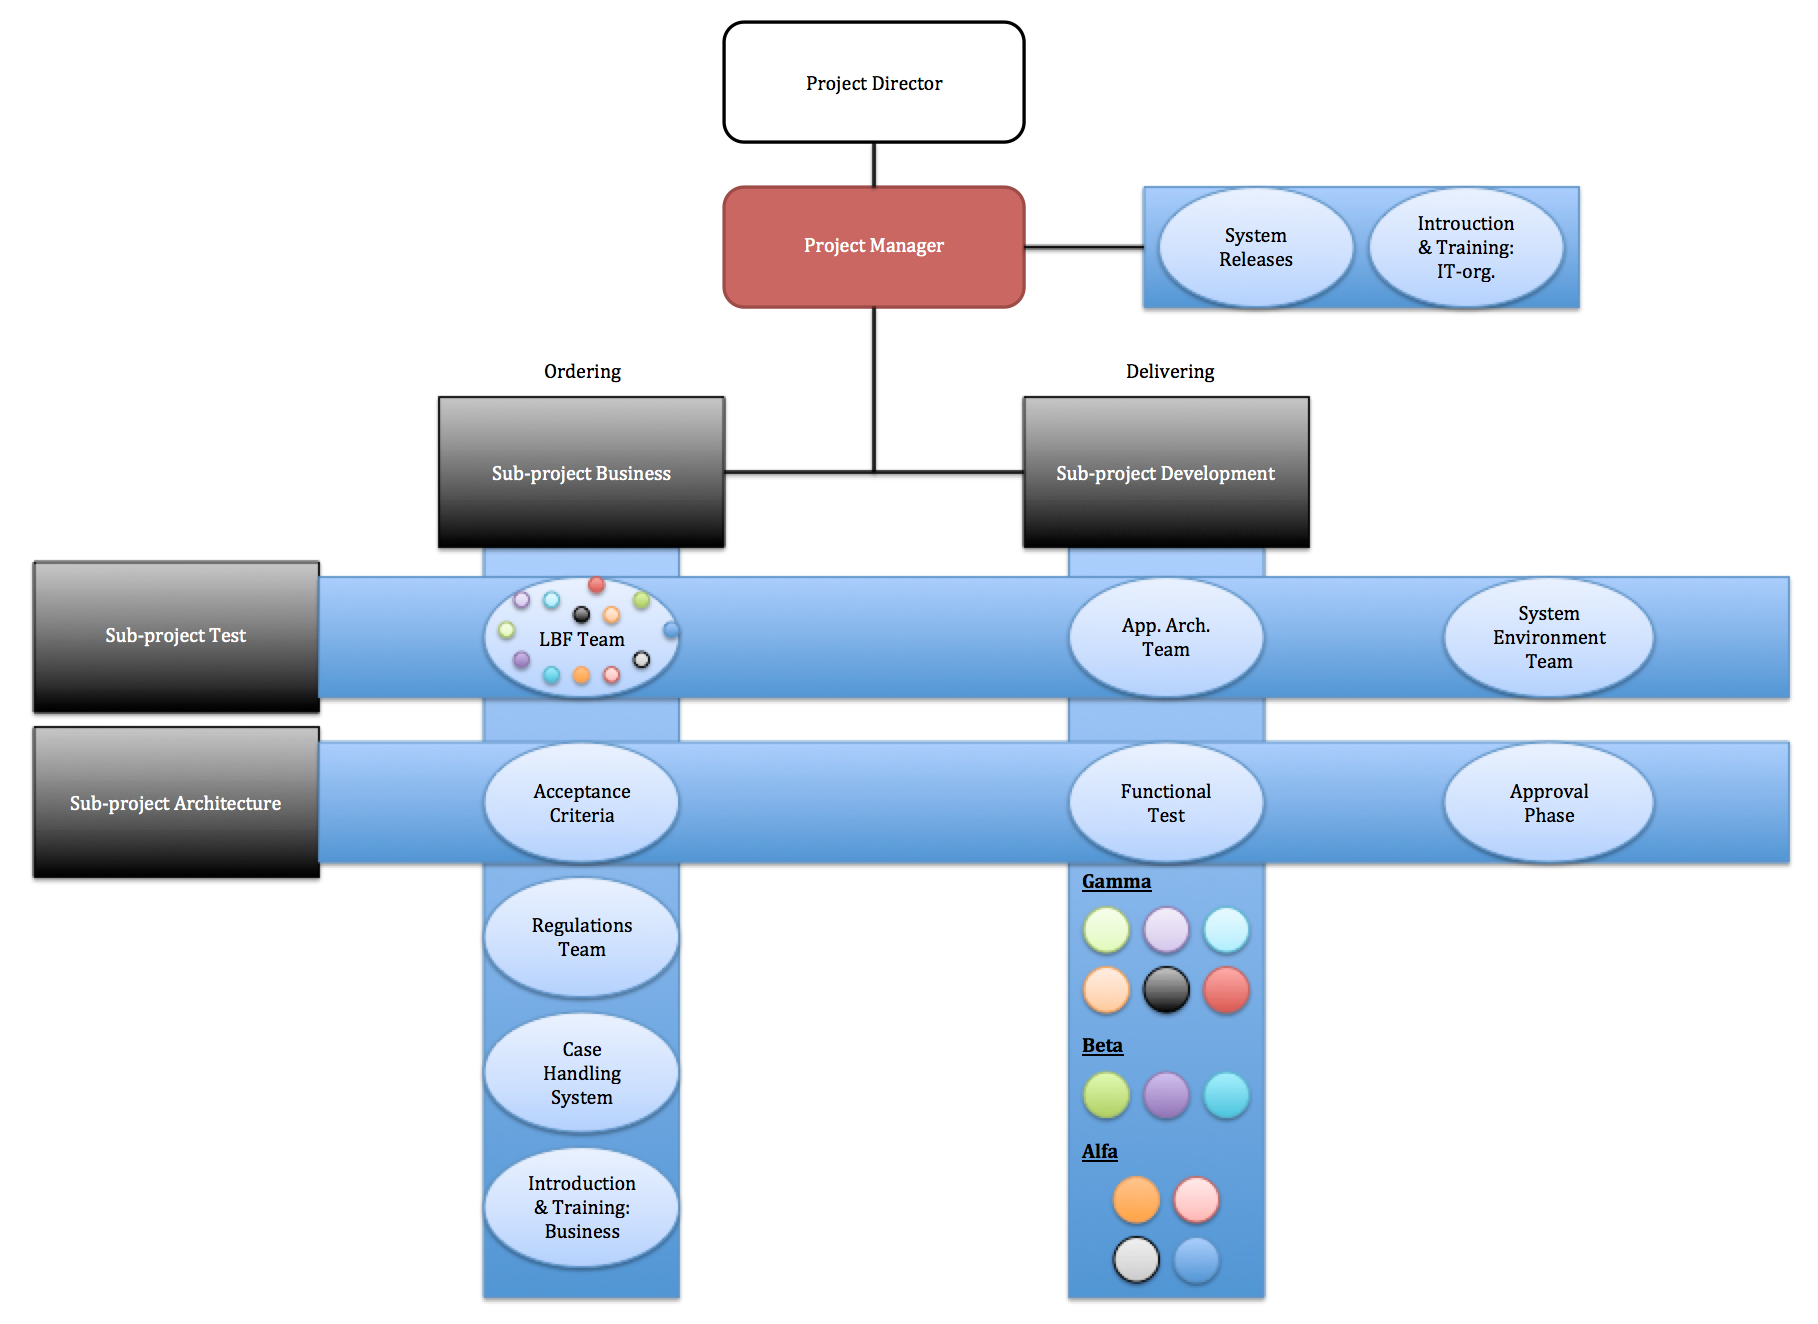
\includegraphics[trim = 40mm 0mm 7mm 0mm,width=180mm]{images/omega_organisation.png}
\caption{Omega-project's organisation.}
\label{omega}
\end{figure}

\begin{figure}[H]
\centering
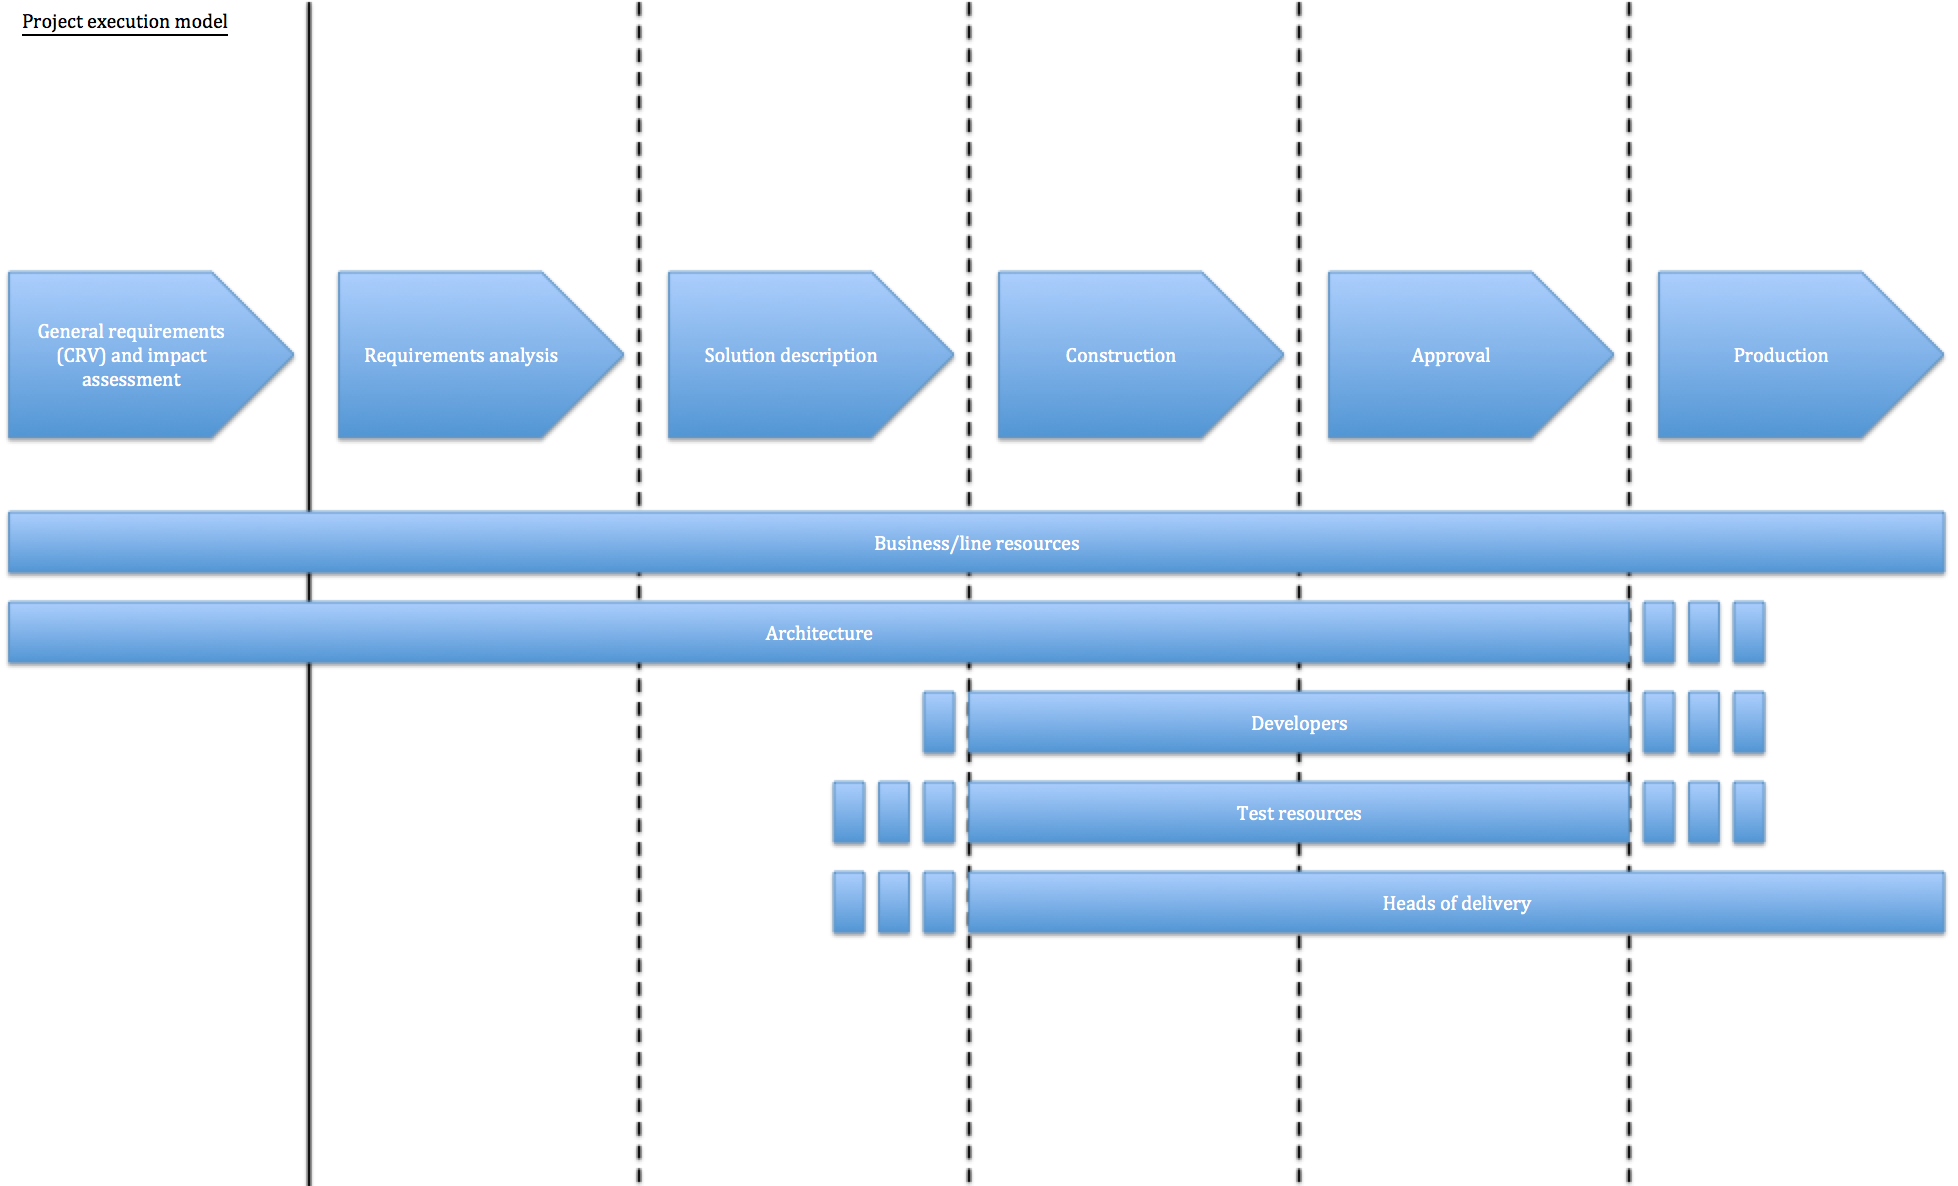
\includegraphics[angle=90, trim = 0mm 0mm 20mm 0mm,width=160mm, height=230mm]{images/execution_model.png}
\caption{Project execution model.}
\label{project_execution}
\end{figure}

\begin{figure}[H]
\centering
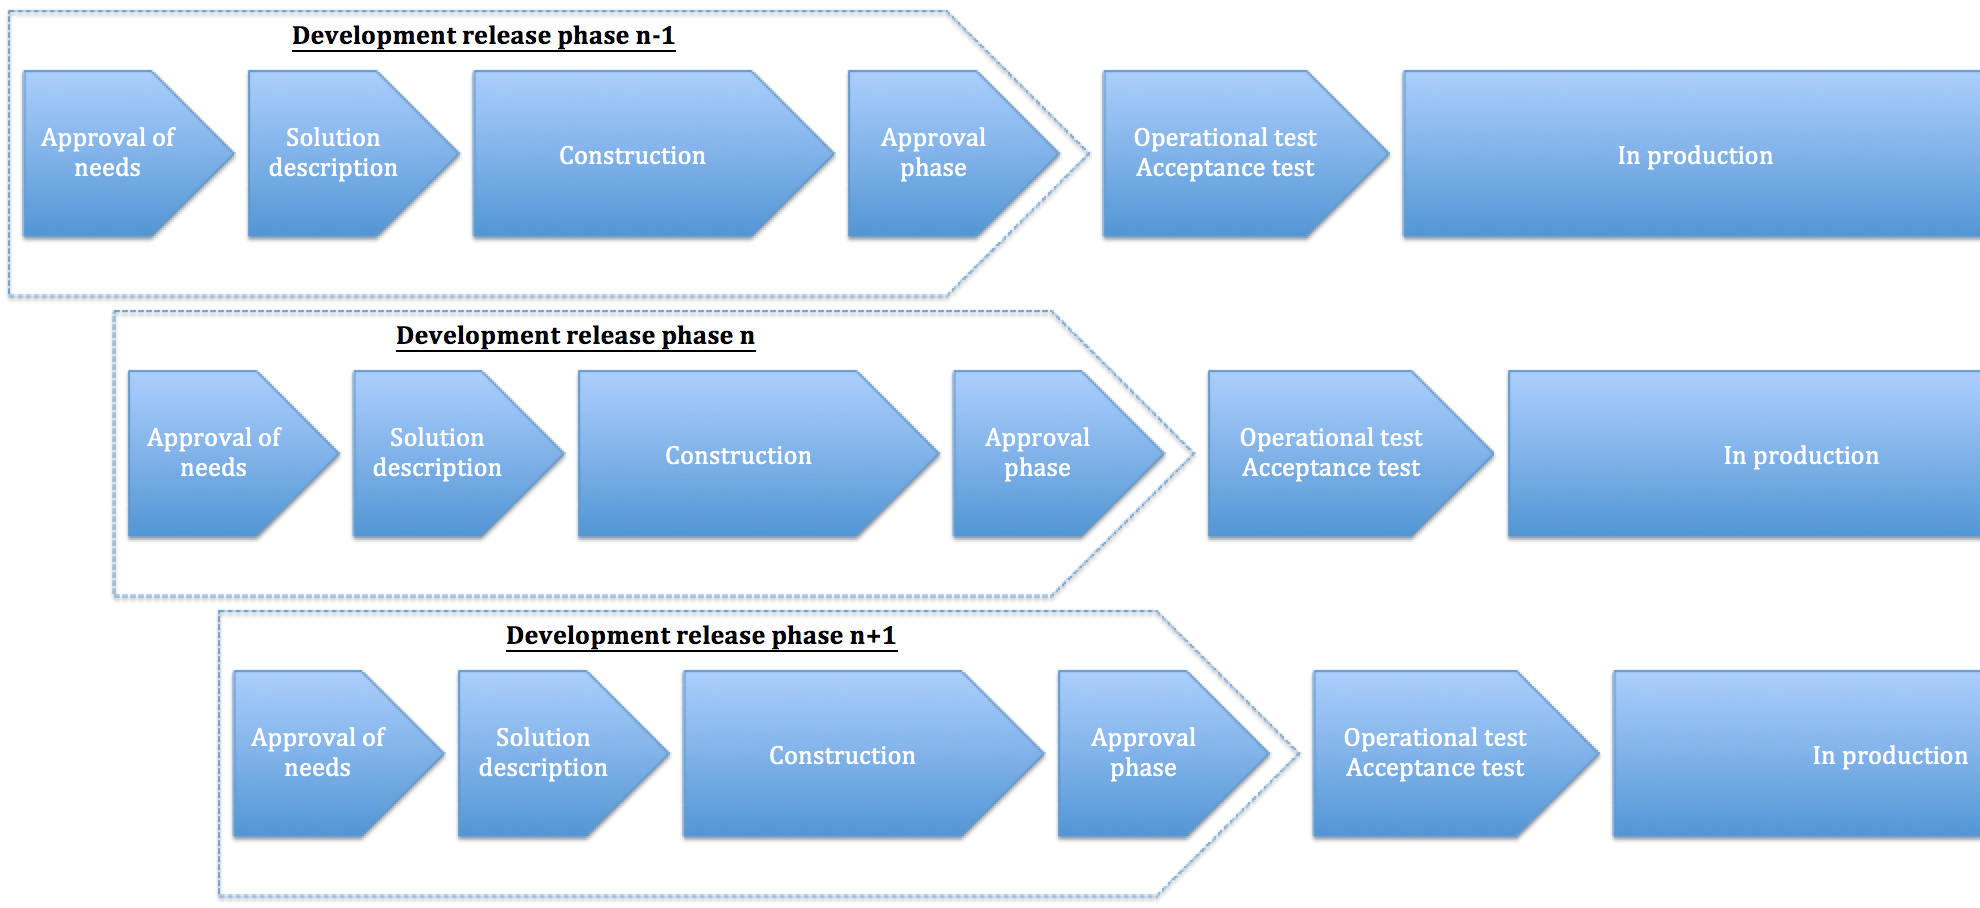
\includegraphics[angle=90, trim = 0mm 0mm 20mm 0mm,width=160mm, height=230mm]{images/initial_development_process}
\caption{Initial development process.}
\label{initial_development_process}
\end{figure}

%\begin{table}[H]
\begin{center}
    \begin{longtable}{| p{6cm} | p{9cm} |}

    \hline \textbf{Coordination mechanism} & \textbf{Description of mechanism} \\ \hline
    \endfirsthead

    \multicolumn{2}{c}%
{{\bfseries \tablename\ \thetable{} -- continued from previous page}} \\ \hline
    \textbf{Coordination mechanism} & \textbf{Description of mechanism} \\ \hline
    \endhead

    \multicolumn{2}{|r|}{{Continued on the next page\ldots}} \\ \hline
    \endfoot

   \endlastfoot

    Metascrum & A meeting similar to Scrum of Scrums but with less details which was held twice per week. Attending the metascrum was the project leaders and all the sub-project leaders from test, architecture, business and development. A ``technical metascrum'' was tried, but was shortly shut down after initiation. \\ \hline
    Planning day & The planning day was a form of kick-off for each sprint iteration where the project members met up with the project owner. The planning day was performed on three levels: project, organisation (Alpha, Beta and Gamma) and team. A rough sketch of the focus areas and work to be performed in the coming sprint was presented with a distribution towards each of the three organisations by the project owner. After this the organisations distributed the work on their respective teams, and lastly the teams got together separately and worked out a contract with estimated work to be performed which was delivered to the project owner team. Before the planning day commenced the developers also had a ``developer forum'' where development-oriented information and discussion was carried out. This was however held on an organisation basis, and not across the three organisations. \\ \hline
    Demo & Demo presentations were held by all Scrum teams at the end of each sprint iteration where everyone could attend. Each team was allocated approximately 10 minutes. There were also larger demo presentations for the project owner when a new release was finished. Some teams in addition started performing smaller demo sessions within the iterations to get rapid feedback. \\ \hline
    Pre-planning day & Before the ``planning day'' was carried out a pre-planning day was performed. Here typically different types of architects (especially functional architects) and the project owner (as well as some other members of the project owner's team) met to create a rough classification and allocation of work to the different Scrum teams for the coming sprint iteration. The allocated work was listed in a prioritised manner. \\ \hline
    Dependency meeting & A meeting held between all Scrum masters from the Alpha, Beta and Gamma teams. This meeting was held on the ``Planning day'' where the focus was on discovering dependencies across Scrum teams. However, these meetings faded away early on because of the dependencies being discovered and handled elsewhere. \\ \hline
    Solution description / ``Master plan'' & At the start of the Omega-project a larger solution description phase was performed involving a lot of architects (as can be seen from figure \ref{project_execution}). This lead to a ``master plan'' for the project and was documented in an issue tracker program called Jira. The ``master plan'' was continuously altered throughout the course of the development phase as outlined in figure \ref{initial_development_process}. In the solution description meetings important aspects were discussed such as coordination across organisations and management of activities. An example of what came out of these meetings was a dependency map of the whole Omega-project, which was in constant change. Part of the solution description meetings were also negotiation and estimation meetings which were important for the contract for each release. \\ \hline
    Jira and Wiki/Confluence & Different programs and forums were used for documentation and tracking within the project. In Jira all user stories and epics were located, and different information about the project and current sprint iteration could be seen on different levels, such as project and team level. The dependency map for the whole Omega-project was also located in Jira. Confluence was the main program used as a wiki. Here solution descriptions, team routines, routines across teams, system documentation, check lists, retrospectives, architectural guidelines, functional test etc. were all located. \\ \hline
    Open-space & An arena held on a voluntary and need basis, which was used for exchanging experiences. Only used during a few of the releases. Participants suggested the topics beforehand, leading to agendas for open-space sessions. \\ \hline
    Jabber & Jabber was introduced as an instant messaging service in the Omega-project after being identified as something needed in one of the Open-space sessions. Project members could ask both formal questions, e.g., technical questions, and informal questions or activities, e.g., wine lotteries. \\ \hline
    Lunch seminars & Kind of similar to the ``open-space'' sessions. Typically two to three topics were held by project-personnel on relevant and interesting topics, often regarding themes correlated to the current situation of the project. As with the ``open-space'' session these seminars were also held on a certain period of the project before fading away. \\ \hline
    Front-end meeting & The front-end developers worked with a complex framework called Flex. Because of this a lot of coordination had to be handled between teams working with this framework from all organisations. Therefore, front-end meetings where held were typically the most prominent Flex-developers were present. \\ \hline
    Technical architecture forum & At the technical architecture forum all technical architects met up to discuss what was to be done in the coding base to prevent coordination issues. These meetings were slowly fading away because the need was covered in other arenas. \\ \hline
    Architecture council & At these gatherings an architecture council listened to all team architects present their respective team's tasks for each sprint iteration. \\ \hline
    Business meeting & The business part of the Omega-project was coordinated through meetings where the business architects from Alpha, Beta and Gamma met up with the business unit from the project owner. Here the sprint iteration queue, and the current status of the project and sprint was presented. This meeting was held around one time each week or every other week. \\ \hline
    Bug-board discussion & The quality assurance unit with its testers had frequent meetings around bug-boards, especially after new releases and around acceptance testing. In the period after a new release these meetings were often held on a daily basis. Here all the bugs were gone through and allocated to the responsible Scrum team in either Alpha, Beta or Gamma. \\ \hline
    
    \caption{Coordination mechanisms used across the whole Omega-project.}
    \label{cmuatwo} 
    \end{longtable}
\end{center}
%\end{table}

\begin{center}
    \begin{longtable}{| p{6cm} | p{9cm} |}

    \hline \textbf{Coordination mechanism} & \textbf{Description of mechanism} \\ \hline
    \endfirsthead

    \multicolumn{2}{c}%
{{\bfseries \tablename\ \thetable{} -- continued from previous page}} \\ \hline
    \textbf{Coordination mechanism} & \textbf{Description of mechanism} \\ \hline
    \endhead

    \multicolumn{2}{|r|}{{Continued on the next page\ldots}} \\ \hline
    \endfoot

   \endlastfoot

    Scrum of Scrums (SoS) & Scrum of Scrums were meetings held by all organisations (Alpha, Beta and Gamma) ranging from two to three times per week. In these meetings all Scrum masters from the corresponding organisation, as well as project management (project leader, test leader, head technical architect, head functional architect, business leader and development leader). The main goal of the SoSs was to identify and handle obstacles. There were also held a few SoS meetings across organisations to handle potential changes to the contracts. \\ \hline
    Technical corner & The ``technical corner'' was a meeting Beta had in an early stage of the project. It was held on Fridays for about 1-1,5 hour. Here team architects presented important themes for the Beta-members. After a while it was shut down because of lack of interest and topics. \\ \hline
    Experience forum & The experience forum was an arena established in the Alpha-organisation for exchanging experiences. Here Scrum masters and the development manager met to discuss topics such as retrospectives, the planning day, and how work was performed by the Alpha-organisation's Scrum teams. It could be seen as a coaching-session with exchange of ideas and thoughts. \\ \hline
    Retrospective & Different levels at Alpha (team, solution description and project management), Global retrospektiv testet ut på Beta \\ \hline
    Technical architecture meeting & \\ \hline
    Functional architecture meeting & \\ \hline
    Supplier meeting & Alpha \\ \hline
    Meeting about queue & Alpha \\ \hline

    \caption{Coordination mechanisms used across teams within the specific organisations (Alpha, Beta and Gamma) in the Omega-project.}
    \label{cmuasito}
    \end{longtable}
\end{center}

\begin{center}
    \begin{longtable}{| p{6cm} | p{9cm} |}
   
    \hline \textbf{Mechanism/Aspect} & \textbf{Description} \\ \hline
    \endfirsthead

    \multicolumn{2}{c}%
{{\bfseries \tablename\ \thetable{} -- continued from previous page}} \\ \hline
    \textbf{Coordination mechanism} & \textbf{Description of mechanism} \\ \hline
    \endhead

    \multicolumn{2}{|r|}{{Continued on the next page\ldots}} \\ \hline
    \endfoot

   \endlastfoot 

    Stand-up &  \\ \hline
    Board discussion & An important aspect for coordination, discussion and status updates in the project was the frequent use of whiteboards. The stand-up meetings were for instance held around these boards, and on these boards the workload for each sprint iteration was put up and updated as the sprint moved along. The backside of the boards were left open to carry out informal discussion when needed. \\ \hline
    Co-location & \\ \hline
    Informal communication & \\ \hline
    Trust & \\ \hline
    Joint coffee break & Alpha (generelt?) \\ \hline
    Pair-programming & \\ \hline
    Self-organising & \\ \hline
    Rotation of team members & \\ \hline
    Rotation of team placement & \\ \hline
    Alfa/Beta-personnel placed in Gamma teams & \\ \hline
    Project management in same location & ``Walking around, talking around'' \\ \hline
    Continuous planning & \\ \hline
    3-level hierarchy from product owner & \\ \hline

    \caption{Other coordination mechanisms and important aspects.}
    \label{ocmaia}
    \end{longtable}
\end{center}